% !TEX encoding = UTF-8 Unicode

% Beispiel für ein LaTeX-Dokument im Format "seminarvorlage"
\documentclass[ngerman]{seminarvorlage}
% ngerman = Deutsch in neuer Rechtschreibung, alternativ english

\usepackage[utf8]{inputenc} % Kodierung der Umlaute
\usepackage{babel} % automatische Sprachanpassung, Sprache siehe oben
\usepackage{cleveref} % für bequeme Referenzen, siehe \cref unten
\usepackage{amsmath}
\usepackage{amsfonts}
\usepackage{amssymb}
\usepackage{graphicx}
\usepackage{color}
\usepackage{listings}
\lstset{
  frame=trb,
  language=C,
  basicstyle=\small,
  breaklines=true, 
  numbers=left,              
  stepnumber=1,                     
  numberfirstline=false,
  tabsize=2,
  commentstyle=\color{magenta}, 
  keywordstyle=\color{blue},
  stringstyle=\color{red}
}


\begin{document}

% Unbedingt angeben: Titel, Autoren, E-Mail
% Freiwillig: Adresse
\title{The Completely Fair Scheduler}
\numberofauthors{2}
\author{
  \alignauthor Lukas Essig\\
    \email{lukas.essig@studium.fernuni-hagen.de}
  \alignauthor Peter Müller\\
    \email{peter.müller@studium.fernuni-hagen.de}
}

\maketitle

\abstract{ tbd. } % Trennhilfe \- manchmal nützlich

\keywords{Linux, CFS, Rot-Schwarz-Baum, Scheduling, completely fair}

% Section-Überschriften werden in GROSSBUCHSTABEN umgestellt
\section{Einleitung}
TODO am Ende: hier folgen einleitende worte, woher der cfs kommt, seit wann im kernel, was das ziel dieses papers ist, was abgegrenzt wird,

\section{Grundlagen zum Scheduling}
In diesem Abschnitt wird der Begriff Scheduling im Allgemeinen und konkret im Bezug auf Prozess-Scheduling definiert und anhand von Beispielen exemplarisch konkretisiert. 
Darauf folgend werden die Kriterien wiederholt, die durch effizientes Scheduling optimiert werden.
Ebenso erfolgt eine Einführung in die Datenstruktur \textit{Rot-Schwarz-Baum} sowie dem \textit{completely fair} Prinzip.

\subsection{Scheduling}\label{s:scheduling}
In der Fachliteratur wird der Begriff Scheduling mit zwar unterschiedlichen Begriffen, jedoch gleicher Bedeutung definiert. Michael Pinedo beschreibt Scheduling in seinem Werk \cite{mpinedo} folgendermaßen:
\begin{quote}
\textit{"`Scheduling is a decision-making process [...]. It deals with the allocation of resources to tasks over given time periods and its goal is to optimize one ore more objectives."'}
\end{quote}
So definiert er Scheduling als einen Entscheidungsprozess, der sich mit der zeitlichen Zuteilungen von Re"-ssourcen zu Aufgaben beschäftigt. Dabei ist das Ziel, ein oder mehrere Eigenschaften zu optimieren. Ferner erklärt er, dass die Ressourcen und Aufgaben in einer Organisation unterschiedliche Formen annehmen können. Ressourcen können beispielsweise Maschinen in einer Fertigungsanlage, Landebahnen auf einem Flughafen oder Verarbeitungseinheiten in einem Rechnersystem sein. Die Aufgaben wären analog Operationen in der Fertigunsanlage, Start und Landung auf dem Flughafen oder Programmausführungen im Computer. Eigenschaften der einzelnen Aufgaben sind zum Beispiel gewisse Prioritäten, frühester Startzeitpunkt oder ein Ablaufdatum. Die zu optimierende Ziele können ebenfalls viele verschiedene Formen annehmen. Das könnten die Reduzierung der gesamten Ausführungszeit einer Aufgabe sein oder die Minimierung der Anzahl von Aufgaben, die nach ihrer Fälligkeit abgeschlossen wurden.

Eine andere Definition ist von Alessandro Agnetis aus seinem Buch \cite{aagnetis}:
\begin{quote}
\textit{"`[...] by scheduling we mean all actions that have to be done in order to determine when each activity of a set is to start and to complete."'}
\end{quote}
So umfasst seiner Ansicht nach Scheduling diejenigen Tä"-tigkeiten, die zur Bestimmung der Start- und Endzeit einer Aktivität aus einem Set getätigt werden müssen. Den Begriff Job spezifiziert er als Aktivität aus einem Set. So ist jeder Job im Wettkampf mit den anderen um die Nutzung von Zeit und Ressourcen. Als Ressourcen charakterisiert der Autor alles, was zur erfolgreichen Ausführung der Jobs erforderlich ist. Wie M. Pinedo benennt er Scheduling ebenso als einen Prozess, der sich mit der Zuteilung von Ressourcen zu Jobs beschäftigt. Seiner Meinung nach ist ein \textit{Schedule} (Plan) somit durch eine Menge von Startzeiten und zugeteilten Ressourcen bestimmt, der einige vordefinierte Anforderungen erfüllt.\\
Zusammenfassend ergeben die Definitionen aus \cite{mpinedo} und \cite{aagnetis} einen Prozess, der die Planung und Zuteilungen von Ressourcen zu Aufgaben sowie deren Ausführung und Beobachtung beschreibt. Dazu kommt die Einbeziehung sowie Auflösung von Abhängig"-keiten zu anderen Systemen, die Start- und Endzeit einer jeden Aufgabe beeinflussen.

Der Scheduler verwaltet Ressourcen und Aufgaben und erstellt dazu einen optimalen Plan, der sicherstellen soll, dass alle Aufgaben mit ihren Eigenschaften (Startzeit, Ablaufdatum, Priorität) und den benötigten Ressourcen erfolgreich ausgeführt werden. Oftmals ist es nicht einfach, einen optimalen Plan für die gegebenen Anforderungen zu finden. Kriterien, welche durch den Scheduler optimiert werden sollen, sind unten in diesem Abschnitt vorgestellt.\\
\cite{mpinedo} und \cite{aagnetis} zeigen ein Beispiel, in dem die Rolle des Scheduling in einer realen Umgebung illustriert wird:
\begin{description}
\item[Gate-Zuweisung am Flughafen]
An einem Airline-Termi"-nal eines größeren Flughafens gibt es dutzende Gates und hunderte von Flugzeugen, die täglich starten und landen. Sowohl die Gates als auch die Flugzeuge sind nicht identisch. Manche Gates haben räumlich viel Platz, sodass hier auch größere Flugzeuge angekoppelt werden können. Andere sind so gelegen, dass es schwierig ist die Flugzeuge ohne Unterstützung anzukoppeln. Obwohl die Flugzeuge nach einem gewissen Plan ankommen und wieder abheben, gibt es doch zufällige Änderungen, die vom Wetter oder anderen nicht vorhersehbaren Ereignissen beeinflusst werden. Während ein Flugzeug an einem Gate steht, müssen die Passagiere die Maschine verlassen. Diese muss getankt, gereinigt und beladen werden und anschließend die Passagiere des nächsten Fluges einsteigen. Die Abflugzeit ist hier das Ablaufdatum, da bis zu diesem Zeitpunkt alle Aufgaben abgeschlossen sein müssen. Wenn jedoch absehbar ist, dass das Flugzeug nicht am Zielflughafen landen kann, wird es auch nicht abheben. Aus Vorschriftsgründen bleiben die Passagiere dann im Terminal anstatt im Flugzeug. Das Flugzeug würde für eine erweiterte Zeit am Gate stehen bleiben und blockiert es somit für andere.\\
Der Scheduler muss die Flugzeuge so den Gates zuweisen, dass dies physisch möglich ist. Dies impliziert, dass die Flugzeuge an die Gates passen und diese zur geplanten Ankunftszeit auch zur Verfügung stehen. Anforderungen wie die zeitliche Reduktion eines Arbeitsvorgangs für das Airline Personal oder die Reduzierung von Verspätungen müssen dabei optimiert werden.\\
In diesem Beispiel sind die Gates die Ressourcen und die Wartung der Flugzeuge die Aufgaben. 
\end{description}
Im Kontext des \textit{Prozess - Scheduling} definiert Avi Silberschatz in \cite{asilberschatz}, dass dieses dafür verantwortlich ist, die Prozesse aus den Warteschlangen zur Ausführung auszuwählen. Dazu erteilt der Scheduler den Prozessen eine gewisse Zeit lang die CPU in der sie diese Ressource benutzen können. Dabei müssen sowohl im Bezug auf die Prozesse als auch im Bezug auf das Gesamtsystem folgende Ziele optimiert werden \cite{asilberschatz} \cite{rlove}:\\
\textbf{Effizienz} ist im Sinne der Kosten - Nutzen - Relation gleich Ertrag durch Aufwand und ist ein Maß für den Umgang mit knappen Ressourcen (CPU, Fertigungsmaschine, Flughafengate, etc.). Um untätige Zeiten zu vermeiden sollte also eine CPU maximal ausgelastet sein. Ebenso ist es wichtig einen hohen \textbf{Durchsatz} zu erreichen. Für das Scheduling bedeutet dies, dass möglichst viele Aufgaben pro Zeiteinheit ausgeführt werden können. Der Durchsatz hängt de facto stark von der Komplexität der Jobs in Verbindung mit der Masse derer ab. \textbf{Fairness} ist im Kontext des CFS ein sehr wichtiger Faktor (siehe auch \ref{s:fair}): Die Neutralität von Ressourcen sollte gewährleistet sein; jedem Prozess ist im Gesamten die gleiche Prozessorzeit zuzuteilen. Damit wird verhindert, dass eine Instanz \textit{verhungert} und somit nicht dauerhaft vernachlässigt wird. Mechanismen für Fairness sind beispielsweise \textit{Preemption} (Verdrängung) oder \textit{Round Robin} (Zeitscheibenverfahren). 
Aufgaben mit einem Ablaufdatum müssen so eingeplant werden, dass der definierte Zeitpunkt eingehalten wird. Es existieren unterschiedliche Formen von \textbf{Deadlines} bzw. Echtzeitanforderungen: Bei einer \textit{harten} Deadline muss das Ablaufdatum präzise, bei \textit{weicher} Deadline hingegen nur einigermaßen eingehalten werden. Ferner sollte bei jedem Scheduling - Algorithmus versucht werden, die \textbf{Komplexität} so gering wie möglich zu halten, z.B. niedrige Aufwände im Bezug auf die O-Notation. Die Scheduling - Operationen sollten \textbf{einfach und schnell} verfahren sowie transparent sein.  

Für alle Scheduling - Systeme ist es wünschenswert, die Effizienz und den Durchsatz zu maximieren sowie  die Ab"-arbeitungs- und Antwortzeiten zu minimieren. In Batch-Systemen wird Wert auf einen hohen Durchsatz und geringe Antwortzeiten gelegt. In interaktiven (time - sharing) Systemen (bspsw. Betriebssystemen) ist es wichtiger, die Varianz der Antwortzeiten anstatt die durschnittliche Antwortzeit zu minimieren. Realzeitsysteme (z.B. Prozessleittechnik, Motorsteuerung, Robotik) hingegen legen einen hohen Wert auf die Einhaltung der Ablaufdaten und geringe Abarbeitungszeiten \cite{asilberschatz}.\\


%Prozesse können entweder als I/O-gebunden oder als Prozessorgebunden klassifiziert werden (nach \cite{rlove}): Erstere verbringen einen Großteil ihres Lebenszyklus damit, I/O-Ope\-rationen anzuweisen oder darauf zu warten. Bestes Beispiel hierfür sind graphische Userinterfaces wie Texteditoren. Umgekehrt führen prozessorgebundene Prozesse die meiste Zeit ihres Lebenszyklus Code aus und werden häufig durch den Scheduler verdrängt. Ein gutes Beispiel hierfür ist das Tool \textit{ssh-keygen} oder das Rendern eines Videos durch einen Codec.\\
%Viele Scheduler-Algorithmen arbeiten mit einer Kombination aus Prozessprioritäten und Zeitscheiben \cite{rlove}. Bei ersterem ist das Ziel, die Prozesse basierend auf ihrem Wert und dem Anspruch auf Prozessorzeit einzustufen. Prozesse mit höhere Priorität laufen vor Prozessen mit niedrigerer Priorität und bei Gleichheit wird per round-robin-Verfahren ausgewählt. Der Linux-Kernel implementiert da\-für u.a. den sogenannten \textit{nice}-Wert in einem Interval von -20 bis +19 und dem Standardwert 0. Höhere nice-Werte korrespondieren zu niedrigeren Prioritäten. Umgangssprachlich ist der Prozess  \textit{netter} zu anderen Prozessen. Prozesse mit niedrigerem nice-Wert erhalten einen größeren Anteil an der CPU. \\
%Über Zeitscheiben wird im Allgemeinen gesteuert, wie lange ein ausgewählter Prozess die CPU erhält bevor er vom Scheduler verdrängt wird \cite{rlove}. Dabei ist es wichtig, dass der Wert der Zeitscheiben nicht zu niedrig aber auch nicht zu hoch gewählt wird. Zu kurze Zeitscheiben führen zu einer geringen Effizienz, da beachtliche Zeit im Overhead für Prozesswechsel verloren geht. Zu lange Zeitscheiben führen dazu, dass das System im interaktiven Betrieb zu lange Antwortzeiten besitzt. Hier kommt auch wieder die Kontroverse zwischen I/O-gebundenen und prozessorgebundenen Prozessen zum Tragen, da erstere keine langen Zeitscheiben brauchen dafür aber oft ausgeführt werden wollen und zweitere nach langen Zeitscheiben verlangen, um z.B. die Caches aktuell zu halten.
%Wie der CFS-Scheduler diesen Spagat und die oben genannten Kriterien einhält wird ab Abschnitt \ref{s:cfsmain} erläu\-tert.

\subsection{Parameter von Schedulern}
\textbf{Prozessarten}\\
In der Prozessverwaltung des Schedulers sollen insbesondere zwei Hauptprozessarten berücksichtigt werden. Zum einen gibt es I/O gebundene Prozesse. Diese Prozesse warten stehts auf Eingaben bzw. Ereignisse und führen danach entsprechend Code aus. Daher kann man davon ausgehen, dass diese Prozesse immer nur relativ kurzläufig sind und danach in einer Art Ruhemodus auf weitere Instruktionen warten. Als Beispiel sei z.B. eine GUI zu nennen, welche hauptsächlich nur durch Interaktionen eines Benutzers zur Arbeit aufgefordert wird.

Die zweite Prozessart, welche vom Scheduler behandelt werden muss, ist die prozessorgebundene. Die prozessorgebundenen Prozesse sind hauptsächlich damit beschäftigt, Algorithmen auszuführen und be\-nötigen daher viel Prozessorzeit. Ausserdem laufen diese Prozesse meist solange, bis sie unterbrochen werden.
Es gibt aber auch Mischformen aus beiden Arten. Ein gutes Beispiel ist zum Beispiel das X-Windows System unter Linux. Diese soll eine grafische Interaktivitätsumgebung für den Benutzer bereitstellen und muss aber auch gleichzeitig im Hintergrund einige Berechnung bzw. Dienste dauert ausführen, um zum Beispiel eine gewisse Anwenderfreundlichkeit gewähr\-leis\-ten zu können. 
Auch das Wörterbuch des bekannten Android Betriebssystem stellt eine Mischform beider Prozessarten da. Schon während der Benutzer die einzelnen Buchstaben eingibt, berechnet der passende Prozess im Hintergrund eine Vorschau mit Wörtern um eine Auto\-ver\-voll\-ständigung des Wortes zu erstellen.
Für den Scheduler entstehen in diesem Bereich damit auch zwei wichtige Anforderungen. Zum einem soll er eine schnelle Antwortzeit auf Interaktionen eines Users ermöglichen. Zum andern einen hohen Durchsatz für prozessorgebundene Prozesse bereitstellen.

\textbf{Prioritäten}\\
Damit ein Scheduler eine Auswahl auf die zu aktivierenden Prozesse treffen kann, müssen diese mit Hilfe einer Bewertung attribuiert werden. Diese Möglichkeit wird unter Linux und Unix-artigen Systemen unter anderem mit Zuhilfenahme von Prioritäten erstellt.
Dabei sollen höher priorisierte Prozesse schneller eine Zuteilung bekommen, als die niedrigeren. Gleichwertige werden mit Hilfe eines Round-Robin Verfahrens bzw. mit einer Wartschlange ausgewählt. In manchen Systemen wird sogar die Länge, d.h. wie lange ein Prozess die Zuteilung behalten darf, über die Prioritäts-Attribute verwaltet. Um während des laufenden Systems auch Anpassungen vornehmen zu kön\-nen, ist es den Benutzern sowie dem System gestattet, diese Prioritäten währen der Laufzeit zu ändern.
In Linux sind sogar zwei Prioritäts\-reihen aktiv. Die erste Reihe hat einen Bereich von -20 bis +19 und diese werden als \textit{nice}-Werte bezeichnet. Der Standard liegt hier in der Mitte bei 0. Ein niedriger Wert \textit{nice}-Wert bedeutet, dass der Prozess einen größeren Anteil der zur Verfügung stehenden Prozessorressource zugeteilt bekommt als ein Prozess mit einem höheren \textit{nice}-Wert.
Unter UNIX hat sich dieses Verfahren als Standard durchgesetzt, allerdings kann der \textit{nice}--Wert durch verschiedene Scheduler-Algorithmen auch unterschiedlich verwendet werden.

Die zweite Reihe von Prioritäten, welche in Linux Systemen implementiert ist, sind die Prioritäten der Real-Time-Reihe. Diese haben einen Bereich von 0 bis 99 und werden allgemein den \textit{nice}-Werten bevorzugt. In diesem Umfeld spielt die Höhe des Wertes allerdings eine genau gegensätzliche Rolle,  wie bei den \textit{nice}-Werten. Je höher der Wert in der Real-Time-Reihe, desto höher die Priorität. Unter UNIX wurde mit POSIX.1b ein Standard für diese Anwendung der Realtime Prozesse erstellt, welchen im Linux-Betriebssystem eine hundertprozentig Anpassung gefunden hat \cite{rlove}.

\textbf{Zeitscheiben}\\
Damit mehrere Prozesse scheinbar nebeneinander laufen können bzw. auch überhaupt eine Interaktionmöglichkeit für Benutzer geschaffen werden kann, ist es nötig Prozesse zu unterbrechen und einem anderen wartenden Prozess eine Zuteilung auf die Prozessor\-ressource zu gewähren. Mit Hilfe von Zeitscheiben können Fenster erstellt werden, in denen ein Prozess für eine bestimmte Zeit eine Zuteilung erhält und danach unterbrochen wird.
Aufgabe des Schedulers ist es an dieser Stelle mit Hilfe entsprechender Regeln, solche Zeitscheiben  für die jeweiligen Prozesse zu errechnen. Dabei gibt es folgende Punkte zu beachten:

Werden die Zeitscheiben zu groß bzw. zu lang gewählt, dann leidet die Interaktionsmöglichkeit für den Benutzer und außerdem kann dann der Anschein der Parallel\--Ver\-arbeitung nicht mehr geweckt werden.
Werden sie zu klein gewählt, dann ist der Prozessor nur noch mit den Umschaltvorgänge beschäftigt und die allgemeine Systemperformance wird erheblich gesenkt.

Auch der oben bereits erwähnt Unterschied zwischen I/O und prozessorgebunden Prozessen spielt eine wesentlich Rolle bei der Festlegung der Zeitscheiben. I/O Prozesse benötigen meist nur eine geringe Zeitscheibe, wohingegen die prozessorgebundenen eine größere Zeitscheibe bekommen sollten. Als Standardwert hat sich eine dieser Stelle ein Wert von kleiner als 10ms etabliert. Damit wird eine gute Interaktivitätsmöglichkeit bewahrt.
%
%Der CF-Scheduler verteilt oder berechnet keine direkten Zeitscheiben an die Prozesse. Bei diesem Verfahren wird ein Anteil der CPU berechnet. Die Menge an Zeit, welche ein Prozess zugeteilt bekommt, ergibt sich aus einer Funktion, welche die Gesamtbelastung eines System integriert.
%Dieser Anteil wird direkt beeinflusst durch das Gewicht jedes Prozesses, welches durch den \textit{nice}-Wert ermittelt wird. Hoher Nice-Wert bedeutet weiterhin, dass der Anteil des Prozessor für diesen Prozess vermindert wird. Ein niedriger \textit{nice}-Wert sorgt für eine Erweiterung des Anteil für die CPU.
%Wenn ein Prozess zu bereit überwechselt, muss der Scheduler entscheiden, ob er einen laufenden Prozess unterbrechen darf oder ob er warten muss. Viele Scheduler berechnen diese Erlaubnis aus einer Funktion von Prioritäten und Zeitschlitzen. Der CF-Scheduler hingegen gewinnt diese Entscheidung aus dem aktuellen Verbrauch dieses Prozesses. D.h. wieviel Zuteilung hat der neue Prozess bereits erhalten im Vergleich zum aktuell laufenden Prozess. Wenn dieser Wert kleiner ist, dann wird der laufende Prozess gestoppt und der neue Prozess erhält direkt die Zuteilung.
\subsection{Rot-Schwarz-Baum}\label{s:rb_tree}
Der Rot-Schwarz-Baum stellt eine Erweiterung des bin-ären Suchbaums dar. Er wurde 1972 zum ersten mal von Rudolf Bayer unter dem Namen  \textit{symmetric binary B-Tree} vorgestellt.

Ein binärer Suchbaum eignet sich zum schnellen Finden von Schlüsselelementen. Dabei werden die Elemente nicht wie in einer Liste sequentiell durchsucht, sondern es wird mit einer bestimmten Logik vorgegangen.
Damit kann im Vergleich zur sequentiellen Liste die Laufzeit für verschiedene Operationen verkürzt werden.

Die Anordnung der Elemente wird, wie im Namen bereits enthalten, als Baum vorgenommen. Dabei müssen bestimmte Kriterien für die Anordnung eingehalten werden. Liegt eine bestimmte Anzahl von Elementen vor, die als Binärbaum angeordnet werden sollen, so wird zunächst ein beliebiges Element ausgewählt und als Wurzel gesetzt. Damit kann es allerdings passieren, dass der Baum später nicht ausgeglichen ist und alle Äste unterschiedliche Dimensionen aufweisen. Dies würde zu einer unausgewogenen Suche führen. Daher ist es Sinnvoll an dieser Stelle ein Element mit einem Schlüsselwert zu finden, welcher sich relativ in der Mitte der vorkommenden Werteskala und sich zudem auch bezüglich der Anzahl der Elemente in der Mitte befindet.

Danach werden die anderen Elemente der Reihe nach mit der Wurzel verglichen. Ist das momentan betrachtete Elemente größer als das Wurzelelement, so wird es an der rechten Seite unter der Wurzel angeordnet. Ist es kleiner als die Wurzel, so kommt es auf die linke Seite. Nun kann das nächste Element mit der Wurzel verglichen werden. Wie im obigen Fall wird es, wenn es größer ist, der rechten Seite zugeordnet und wenn es kleiner ist, der linke Seite. An dieser Stelle kann es jetzt passieren, dass auf der ausgewählten Seite bereits ein Blatt bzw. ein Knoten existiert. Hier muss nun ein weiterer Vergleich stattfinden. Wiederum wird geprüft, ob das momentan ausgewählte Element größer oder kleiner ist als dieser Knoten. Dann wird es entsprechend unter dieses Element angefügt. Somit entsteht ein Baum. Wichtig ist in diesem Verfahren, dass jeder Knoten nur maximal zwei Elemente besitzen darf. 

Die Suche nachher im Baum gestaltet sich ähnlich. Soll ein Element im Baum gesucht werden, so wird ein Vergleich an der Wurzel des Baumes gestartet. Ist der Schlüs\-sel des zu suchenden Elements größer, so wird auf die nächste untere Ebene der rechten Seite gewechselt. Ist der Schlüssel kleiner, dann findet der Wechsel entsprechend auf der linken Seite statt. 

Der größte Vorteil dieser Anordnung besteht in der erheblichen Verkürzung der Laufzeit gegenüber beispielsweise einem Listenverfahreren. 
Als Vergleich soll die Laufzeit beim Suchen dienen.
Während beim sequentiellen Suchen in Listen der Maxmimalwert der Laufzeit $O(n)$ betragen kann, mit $n$ als Anzahl der vorhanden Elemente, so wird die Laufzeit beim binären Suchbaum auf maximal $O(h)$ verkürzt, wobei $h$ die Höhe des Baumes ist \cite{tcormen}.

Allerdings kann es auch durch ständiges Löschen und Ein-fügen von Elementen oder aber auch durch eine unvorteilhafte Wahl des Wurzelknotens dazu kommen, dass sich der Baum in einem Ungleichgewicht befindet. Dies bedeutet, dass eine Seite des Baumes erheblich mehr Knoten besitzt als die andere. Dadurch wird sich die Suchlaufzeit auf der einen Seite erhöhen und auf der anderen Seite ver\-kürzen. Im Extremfall wären alle Elemente auf einer Seite hintereinander angeordnet und somit wäre die Laufzeit gleich der einer sequentiellen Liste.

Eine solche Fehlanpassung kann mit Hilfe der Logik eines Rot-Schwarz-Baumes kompensiert werden. Dieser stellt eine Eweiterung des binären Suchbaums dar. Damit ist es möglich, einen sich ständig ändernden Baum in einem annähernden Gleichgewicht zu halten. 

Der Rot-Schwarz-Baum erhält seinen Namen durch ein zusätzliches At\-tri\-but, welches an jeden Knoten an\-ge\-hängt wird und als Wert die Farbe Rot oder Schwarz enthalten kann. 
Mit Hilfe dieses Attributes kann dann der Baum nach bestimmten Regeln bearbeitet werden. Diese Regeln sorgen dafür, dass immer ein grundlegendes Gleichgewicht im Baum herrscht. 
In Abbildung \ref{fig:rbtree} ist der Aufbau eines Rot-Schwarz-Baumes zu sehen.

\begin{figure}[h]
	\centering
	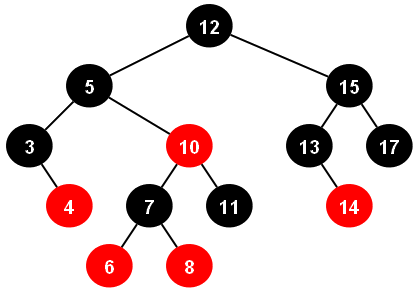
\includegraphics[width=0.45\textwidth]{pictures/redblacktree.png}
%	\caption{RED-BLACK-TREE~\protect\cite{rtoal}}
	\caption{Rot-Schwarz-Baum}
	\label{fig:rbtree}
\end{figure}

 
Nach \cite{tcormen} müssen folgende Regeln eingehalten werden, damit ein Rot-Schwarz-Baum zustande kommt:

\begin{enumerate}
	\item Jeder Knoten ist entweder rot oder schwarz.
	\item Die Wurzel ist schwarz.
	\item Jedes Blatt (NIL) ist schwarz.
	\item Wenn ein Knoten rot ist, dann sind seine beiden Kinder schwarz.
	\item Für jeden Knoten enthalten alle einfachen Pfade, die an diesem Knoten starten und in einem Blatt des Teilbaumes dieses Knotens enden, die gleiche Anzahl schwarzer Knoten. 
\end{enumerate}

Wie bereits Thomas H. Cormen in \cite{tcormen} beweist, kann ein Baum, welcher nach diesen Regeln erstellt wird, eine maximale Höhe von $2lg(n+1)$ erreichen. Damit ergeben sich die Laufzeiten für verschiedene Operation, wie z.B. das Suchen im Baum, auf einen Maximalwert von $O(lg\, n)$.

Beim Einfügen oder Löschen in den Baum werden Verbindungen oder Knoten verändert. Dabei kann es passieren, dass der Baum wieder in ein Ungleichgewicht gerät. 
Um dieser Problematik entgegen zu wirken, werden spezielle Einfüge- bzw. Lösch\-operationen angewendet, welche so konstruiert sind, dass immer die fünf oben genannten Regeln eingehalten werden. 

So müssen innerhalb dieser Einfüge- oder Lösch\-ope\-ra\-ti\-on\-en z.B. Rotationen von Knoten unter bestimmten Bedingung durchgeführt oder die Farben bzw. auch die Zeigerstruktur geändert werden.

Werden die fünf Regeln unter allen Bedingungen und zu jeder Zeit eingehalten, so kann immer die maximale Laufzeit garantiert werden und außerdem können der kleinste und der größte Schlüssel immer direkt auf der linken bzw. auf der rechten Seite gefunden werden.
%Mit den Regeln von RED-BLACK wird mit Hilfe von z.B. Rotationen um das den Parent Knoten, immer für das richtige Gleichgewicht gesorgt.


\subsection{Das completely-fair Prinzip}\label{s:fair}
Die wichtigste Aufgabe eines Schedulers ist die Verteilung von knappen Ressourcen unter einer Menge von Klienten. 
Um dies zu realisieren, wurden bereits viele Anwendungen in Theorie und Praxis entwickelt.
Eine sehr bekannte Entwicklung beruht auf der Idee, jedem Klienten ein eigenes Gewicht zu zuweisen, welche dann je nach Höhe zum Gebrauch der begrenzten Ressource berechtigt.

Diese Verfahren, welches unter anderem unter dem Namen \textit{Proportional Share Scheduling} bekannt sind, wurden bereits vor einigen Jahrzehnten entwickelt und fanden dann z.B. in einem gewichtetem Round - Robin Verfahren Anwendung. Auch unter UNIX fand dieses Verfahren schnell als Scheduler Anwendung mit Hilfe einer Priorität-Steuer\-ung. Dieses Verfahren ist schnell und benötigt immer eine konstante Zeit zum Auswählen des nächsten Klienten. 

Die Proportional - Scheduler können die Verteilung der Ressource hauptsächlich über zwei Wege erreichen:
\begin{enumerate}
	\item Über die Frequenz. Das heißt, wie oft bekommt ein Klient die Zuteilung. Dies kann zum Beispiel realisiert werden, mit einer entsprechenden Positionierung in einer Warteschlange.
	\item Über die Zeit. Dafür wird das Zeitquantum, welches einem Klienten zur Verfügung gestellt wird, entsprechend verlängert oder verkürzt.
\end{enumerate}

Wird die Scheduler - Logik mit Hilfe von Prioritäten gesteuert, entsteht schnell ein entscheidendes Problem. Die Klienten mit den höchsten Prioritäten werden bevorzugt und bei anderen Klienten mit niedrigeren Prioritäten kann der Fall auftreten, dass sie keine Zuteilung mehr bekommen und somit \textit{verhungern}.
Um diese Problematik zu umgehen, wurde mit der Entwicklung alternativer Scheduling Algorithmen begonnen. Ein wichtiges Ziel sollte sein, eine gewisse Fairness unter den Klienten zu erreichen. Damit erhielten diese Verfahren den Namen \textit{Fair Scheduler}. Mit Hilfe dieser Art von Schedulern soll das Problem der ungleichmäßigen bzw. ungerechten Verteilung der Prioritätssteuerung behoben werden.

Eine perfekte Fairness kann nur gebildet werden, wenn die Klienten bewertet werden und aufgrund dieser Bewertung ihre Zuteilung auf die Ressource erhalten.
Eine Möglichkeit für eine solche Bewertung ist ein Vergleich von verbrauchten Kontingent des Klienten zu Verbrauchten Kontingent aller aktiven Klienten in einem bestimmten Zeitraum. 
Dies wird nach \cite{usenix} wie folgt definiert:

\begin{equation}
W_{o,A}(t_1,t_2) = (t_2 - t_1) \frac{S_A}{\sum_i S_i}
\label{eq:perfect_fairness}
\end{equation}

Hierbei ist $S_A$ der proportionale Anteil des Klienten $A$, $S_i$ die Anteile aller aktiven Klienten und $W_{o,A}$ stellt als Ergebnis eine optimale proportionale Menge des Klienten in der Zeit zwischen $t1$ und $t2$ dar.

Im idealen System, wenn alle Klienten ihre Zuweisung gleichzeitig erhalten und ihren geforderten Ressourcenanspruch simultan verbrauchen könnten, wäre es möglich die obige Gleichung für alle Klienten entsprechend aufrecht zu erhalten.
Damit wäre eine \textit{completely-fair} Verteilung gegeben. Allerdings ist dies in der Praxis nicht möglich, da immer nur ein Klienten für die Ressource die Zuteilung bekommen kann.
Um eine Bewertung der aktuellen angewendeten Strategie zur idealen \textit{completely-fair} Strategie zu erhalten, kann ein sogenannter \textit{service time error} mit folgender Formel berechnet werden:

\begin{equation}
E_A(t_1,t_2) = W_{S,A}(t_1,t_2) - W_{o,A}(t_1,t_2)
\label{eq:error_fairness}
\end{equation}

Diese Differenz gibt den Abstand vom gegebenen Algorithmus bzw. der aktuellen Strategie zum optimalen Algorithmus an.
Ist der Abstand positiv, so bekommt der aktuelle Klient mehr Zuteilung als er mit dem idealen Algorithmus bekommen würde. Ist der Abstand negativ, so erhält der Klient im Vergleich weniger.

Je kleiner der Wert aus Formel \ref{eq:error_fairness}, desto mehr erreicht der aktuelle Algorithmus die Funktionsweise des optimalen \textit{completely-fair} Algorithmus.
%Ziel in einer praktischen Lösung im Bezug auf \glqq completely-fair\grqq{} soll es sein, diesen Abstand
 






\section{Der Completely-Fair-Scheduler}\label{s:cfsmain}
Ziel dieses Abschnittes ist es, dem Leser ein grundlegendes Verständnis für die Funktionsweise des CFS zu vermitteln. Es wird konkretisiert, wie dieser Scheduler einen perfekten Multitasking-Prozessor approximiert und welche Datenstrukturen und Funktionen dafür in der Programmiersprache C im Linux-Kernel implementiert sind.

\subsection{Funktionsweise}\label{s:cfs_fktweise}

%hier sollten wir mal reinschauen:
%https://www.ece.ubc.ca/~sasha/papers/eurosys16-final29.pdf
%HAB AUCH SCHON WAS GEFUNDEN...ABER SCHAUE ICH MIR AUCH MAL AN...

%Das Ziel eines  Completely-Fair-Schedulers{} soll es sein, eine gute Annäherung an das Verhalten eines perfekten Multitasking-Prozessor zu errreichen.
Das Ziel eines  Completely-Fair-Schedulers{} soll es sein, eine faire Aufteilung der Ressource Prozessor unter einer Menge von ausführbaren Prozessen zu erreichen.


%Ein perfekter Multi\-tasking-Prozessor würde jedem Prozess immer ein perfektes $1/n$ Verhältnis zuweisen, wobei $n$ die Menge aller Prozesse darstellt."
Im einfachsten Fall, wenn keine Prioritäten unter den Prozessen vergeben werden, ist eine perfekte Aufteilung der Ressource dann gegeben, wenn zu jedem Zeitpunkt jeder Prozess immer eine Zuteilung im Verhältnis $1/n$ erhält, wobei $n$ die Menge aller Prozesse darstellt.
Bei zwei laufenden Prozessen heißt das, dass beide Prozesse zeitgleich mit jeweils 50 Prozent der Prozessorressource arbeiten. Dies ist in der Praxis allerdings nicht möglich, da jeder Prozessor immer nur eine Aufgabe zu einem Zeitpunkt bearbeiten kann.

Unter Linux und UNIXartigen System werden daher den beiden Prozessen Zeitscheiben zugeordnet und es findet eine sequentielle Abarbeitung statt. Anschließend werden die Prozesse abwechselnd mit jeweils 100 Prozent Prozessorzuteilung entsprechend ihrer Zeitscheibe verarbeitet.

%Um mit diesem Prinzip eine Annäherung an einen perfekten Multitasking-Prozessor zu erreichen, müsste man die Zuteilung für jeden Prozess in unendlich kleine Zeitscheiben zerlegen und alternierend dem Prozessor zuweisen.
Je kleiner die Zeitscheiben gewählt werden, desto mehr wird ein nahezu zeitgleiches Abarbeiten der anstehenden Prozesse erreicht.
Wird zu einer beliebigen Zeit eine Messung der bereits zugeteilten Anteile der Prozesse durchgeführt, sieht es tatsächlich so aus, als wür\-den alle Prozesse ihr Quantum gleichzeitig verbrauchen.
Allerdings hat diese Methode eine erheblichen Nachteil. Ein einziger Umschalt\-vorgang be\-nötigt selbst z.B. durch Ein- und Auslagerung der verschieden Daten im Speicher, wieder einen großen Teil der Prozessorleistung. Dadurch entsteht ein sehr schlechtes Verwaltungs- zu Verarbeitungs\-verhält\-nis und somit ist der Scheduler sehr uneffizient. Damit es nicht zu dieser Problematik beim CFS Scheduler kommen kann, wird eine minimale Zeitscheibe festgelegt. Diese minimale Zeitscheibe wird im Kernel als \textit{sysctl\_sched\_min\_granu\-larity} bezeichnet \cite{paperfairness}.
Somit wird an dieser Stelle sichergestellt, das der Verwaltungsaufwand zum Umschalten der Prozesse die Bearbeitungszeit der Prozesse im Prozessor nicht übersteigt.


%Mit dem CFS - Scheduler muss nun eine Umgebung geschaffen werden, welche stark an der des idealen Multitasking-Prozessor anlehnt und wiederum aber auch die Effizienz zur Ausnutzung der Prozessorressource in einen akzeptablen Bereich bewegt.
Anders als bei den prioritäts\-bestim\-mten Scheduler, welche über Zeitscheiben und Warte\-schlan\-gen die Prioritäten verwalten, berechnet der CFS - Scheduler die Zuteilung im Bezug zu allen anderen Prozessen, welche sich in der entsprechenden Warteschlange des Prozessors befinden. Der  \textit{nice}-Wert, welcher bereits in älteren Scheduler\-ver\-fahren für die Erstellung der Zeitscheiben zuständig war, wird jetzt verwendet, um den Prozessen ein Gewicht zuzuordnen. Ist der  \textit{nice}-Wert hoch, was eine niedrige Priorität bedeutet, so bekommt der Prozess auch ein niedriges Gewicht zugeteilt. Andersherum bekommt der Prozess ein hohes Gewicht, wenn der  \textit{nice}-Wert niedrig ist.

Mit Hilfe dieses Gewichtes wird dann das  Completely-Fair-Prinzip [s. Kapitel \ref{s:fair}] angewendet. 

Analog der Formel \ref{eq:perfect_fairness} wird zunächst mit Hilfe des ermittelten Gewichtes und der zu berechneten  Periode eine ideale Zeitscheibe errechnet. Dies geschieht nach \cite{paperfairness} mit folgender Formel:  

\begin{equation}
slice = \frac{se\rightarrow load.weight}{cfs\_rq\rightarrow load.weight} * period
\label{eq:slice}
\end{equation}

Hierbei ist \textit{se$\rightarrow$load.weight} das Gewicht des Prozesses aus dem entsprechendem \textit{nice}-Wert, welches durch ein von dem Kernel bereit gestelltes Array \texttt{prio\_to\_weight[]} ermittelt wird. In \cite{nikita} wird der Inhalt des Arrays mit folgenden Werten angegeben:

\begin {table}[h]
\begin{center}
\begin{tabular}{r|rrrrr}
 &	\multicolumn{5}{c}{\textit{Gewichte}} \\
	\hline\hline
	\\[\dimexpr-\normalbaselineskip+2pt]
	\textit{nice} & &+1	&	+2	& +3	& +4	\\
	\hline
    \\[\dimexpr-\normalbaselineskip+2pt]
	-20	&	88761	&	71755	&	56483	&	46273	&	36291	\\
	-15	&	29154 	&	23254 	&	18705 	&	14949 	&	11916	\\
	-10	&	9548	&	7620	&	6100	&	4904	&	3906	\\
	-5 	&	3121 	&	2501 	&	1991 	&	1586 	&	1277	\\
	0	&	1024 	&	820		&	655		&	526		&	423		\\
	5 	&	335 	&	272		& 	215		&	172		&	137		\\
	10	&	110		&	87 		&	70 		&	56 		&	45		\\
	15 	&	36 		&	29 		&	23 		&	18 		&	15	 	\\		
\end{tabular}
\caption {\textit{nice}-Wert zu Gewicht} \label{tab:nice2weight} 
\end{center}
\end{table}

   
Die Variable \textit{cfs\_rq$\rightarrow$load.weight} ist die Summe aller Gewichte der momentan aktiven Prozesse der Warte\-schlan\-ge.
\textit{period} ist der \textit{Zeitschlitz}, für welchen eine Bewertung mit Basis auf die idealen Zeitscheiben der aktuellen Prozesse vorgenommen werden soll. Dieser Wert ist nicht konstant und einstellbar. Erreicht z.B. die Anzahl der lauf\-fähigen Prozesse eine kritische Grenze, so muss der Wert von \textit{period} erhöht werden. 
Diese Grenze wird im Kernel mit Hilfe der Variable \textit{nr\_latency} ermittelt. Diese Variable setzt sich aus dem Verhätlnis von \textit{period} und der minmalen Zeitscheibe zusammen \cite{paperfairness}.

\begin{equation}
nr\_latency = \frac{sysctl\_sched\_latency}{sysctl\_sched\_min\_granularity}
\label{eq:nr_latency}
\end{equation}

Somit gibt die Variable \textit{nr\_latency} die maximal mögliche Anzahl von Prozessen mit gegebenen Parametern vor. Über\-steigt nun die Anzahl der aktuell lauffähigen Prozesse diesen Wert, so muss der Wert von \textit{period}, bzw. in Formel \ref{eq:nr_latency} ensprechend \textit{sysctl\_sched\_latency}, erhöht werden.

Im anschließendem Schritt soll eine faire Auswahl auf den nächsten ausführbaren Prozess getroffen werden. Dies geschieht mit einer weiteren Bewertung der Prozesse im Bezug zu ihrer bereits ausgeführten Zeit. 
Dazu dient im Algorithmus die Variable \textit{virtual runtime}. In \cite{mjones} wird die \textit{virtual runtime} definiert als Menge der CPU-Zeit, die einer gewissen Aufgabe zugeordnet worden ist. Umso kleiner der Wert für \textit{virtual runtime} ist, desto höhere ist die Dringlichkeit dieser Aufgabe den Prozessor für sich zugewiesen zu bekommen. Ebenso beschreibt \cite{mjones} die Funktionalität von CFS, dass eine gewisse \textit{Sleeper-Fairness} implementiert ist: Aufgaben, die zu einem Zeitpunkt nicht lauffähig sind (z.B. beim Warten auf I/O"--Operationen) erhalten einen vergleichbaren Anteil am Prozessor, wenn sie diesen benö"-tigen.\\
Die \textit{virtual runtime}-Variable wird aus dem Verhältnis von bereits absolvierter Zeit zu dem ermitteltem Gewicht des Prozesses gebildet und ist für die Dauer der Ausführungs"-zeit für jeden Prozess ständig steigend \cite{rlove}. 

Nach \cite{paperfairness} wird \textit{virtual runtime} mit folgender Formel ermittelt:

\begin{multline}
vruntime \mathrel{+}= \frac{delta\_exec}{se\rightarrow load.weight} * NICE\_0\_LOAD \\ = \frac{period}{cfs\_rq\rightarrow load.weight} * NICE\_0\_LOAD
\label{eq:vruntime}
\end{multline}

Hierbei stellt \textit{delta\_exec} die bereits ausgeführte Zeit der jeweiligen Prozesses dar und \textit{NICE\_0\_LOAD} ist der Einheitswert der Gewichte, welcher das Gewicht des \textit{nice}-Wertes 0 darstellt.  
%welcher aus einer statischen 10-bit Dualzahl besteht $(2^{10}=1024)$ \cite{paperfairness}. 
Mit Hilfe des ersten Terms aus Formel \ref{eq:vruntime} wird die aktuelle virtuelle Laufzeit des jeweiligen Prozesses bestimmt. Der zweite Term dient zur Bestimmung der allgemeinen virtuelle Laufzeit, welche jeder Prozess nach Ablauf der Periodenzeit \textit{period} für diesen Zeitabschnitt erreicht haben soll. Dieser Wert soll nach Ablauf der Periodenzeit für alle Prozess gleich sein.

Mit dieser neuen Variablen können nun die Prozesse entsprechend ihrer Laufzeit und ihrem Gewicht bewertet und eine Rangfolge erstellt werden. Dazu wird an dieser Stelle der Rot-Schwarz-Baum [s.Kapitel \ref{s:rb_tree}] verwendet. Die Prozesse werden nach ihrem \textit{virtual runtime}-Wert in den Baum einsortiert. Dabei steht der Prozess mit der kleinsten \textit{virtual runtime} am weitesten links und kann nun durch den Scheduler ohne lange Suchzeiten ermittelt und als nächster auszuführender Prozess ausgewählt werden. 

Stehen zum Beispiel drei lauffähige Prozesse  mit \textit{nice}-Werten $0$, $1$ und $2$ und entsprechenden Gewichten von $1024$, $820$ und $655$ in einer Warteschlange für einen Prozessor.
Dann ergeben sich die idealen Zeitscheiben bei einer Periode von 20ms mit Formel \ref{eq:slice} zu $8.2ms$, $6.6ms$ und $5.2ms$. Ermittelt man nun dazu passend die \textit{virtual runtime}-Werte und zwar so, dass jeder Prozess seine Zuteilung für diese Periode vollständig ausgenutzt hat, so wird ersichtlich, dass alle Prozesse nun den gleichen \textit{virtual runtime}-Wert von ca. $8*10^{-6}$ besitzen. Damit wird eine faire Aufteilung mit Be\-rück\-sichtigung der \textit{Prioritäten} gewährt.

%Jeder Prozess er\-hält eine Zeitscheibe, welche proportional zum eigenen Gewicht im Verhältnis zu den Gewichten aller Prozesse ist. Die Wahl des nächstes Prozesses fällt immer auf den Prozess, welcher bis zu diesem Zeitpunkt die geringste Zuteilung des Prozessors erhalten hat.
%Zur Berechnung einer Zeitscheibe, setzt der CFS - Scheduler eine sogenannte „targeted latency“. Diese stellt einen Richtwert für die verfügbare Zeit aller anstehenden Prozesse dar, welcher äquivalent im perfekten Multitasking erreicht würde.

%Wenn zum Beispiel eine „targeted latency“ von 20ms errechnet wird und zwei Prozesse mit dem gleichen  \textit{nice}-Wert in der Warteschlange stehen, wird jedem Prozess eine Zuteilung von 10ms gewährt.

%Ein Problem ergibt sich bei dieser Anwendung, wenn die Anzahl der wartenden Prozesse gegen unendlich läuft. Damit würde die zugewiesene Zeit gegen Null laufen und es würde kein Prozess mehr die Berechtigung einer Zuteilung erhalten. Um dieses Problem zu umgehen, wird eine minimale Granulität eingeführt ,welche normalerweise mit einer Millisekunde gewählt wird. Das heißt jeder Prozess erhält immer mindestens eine Zuteilung von einer Millisekunde, egal wie groß die Menge der anstehenden Prozesse zu diesem Zeitpunkt ist. Dadurch wird allerdings das „faire“ Verhalten des Schedulers beeinträchtigt. 

%Auch findet eine weitere Unterscheidung zur Nutzung der  \textit{nice}-Wert statt. Wurde zuvor der absolute  \textit{nice}-Wert für eine Prioritätsermittlung benutzt, so spielt jetzt nur noch der relative Abstand zum nächsten  \textit{nice}-Wert eine Rolle.

%Ein passendes Beispiel ist in \cite{rlove} illustriert. Gegeben ist ein Zustand mit zwei Prozessen. Ein Prozess hat den  \textit{nice}-Wert 0, der andere den  \textit{nice}-Wert 5. Damit würde sich eine Prozessorzuteilzeit von 15ms für den Prozess mit  \textit{nice}-Wert 0 und eine Zuteilzeit von 5ms für den Prozess mit  \textit{nice}-Wert 5 ergeben.
%Im Vergleich dazu hätte man einen weiteren Zustand mit wiederum 2 Prozessen, aber dieses mal mit den  \textit{nice}-Werten 10 und 15. Hier würde das selbe Ergebnis mit 15ms und 5ms zustande kommen. Damit wird gezeigt, dass die Höhe des  \textit{nice}-Wertes nur noch die geometrische Differenz ändert.

%Anhand dieser Erläuterung kann gesehen werden, dass der CFS - Scheduler nur eine Annäherung an ein perfektes faires Scheduling erreicht. Das große Problem der CFS - Scheduler ist eine übermäßige Menge an Prozessen. Wird diese Menge in einem gewissen Rahmen gehalten, so kann der CFS - Scheduler das  completely-fair -Prinzip gut erreichen. 

\subsection{Implementierung im Linux-Kernel}\label{s:cstructs}
Im folgenden Abschnitt werden Datenstrukturen und Funktionen der Programmiersprache C aus dem Linux-Kernel vorgestellt, die für Scheduling-Aktivitäten des CFS genutzt werden. Dies umfasst die gewichtete Berechnung der genutzten Prozessorzeit sowie den nötigen Aktionen zur Prozessselektion (Einfügen, Lö"-schen und Auswahl eines Prozesses). Die Erläuterungen folgen den Diskussionen aus \cite{rlove}. Aus Gründen der Über"-sicht"-lichkeit wird hier auf die Darstellung von Sourcecode verzichtet. Diese können z.B. im Internet unter \footnote{\url{https://github.com/torvalds/linux/tree/master/kernel/sched}} eingesehen werden.

Wie in Kapitel \ref{s:cfs_fktweise} erläutert, ordnet der CFS jedem Prozess die gewichtete, bereits genutzte Prozessorzeit \textit{virtual runtime} zu. \\
In der ersten Version im Kernel 2.6.23 wurde die \textit{virtual runtime} aus der Kombination einer systemweiten \texttt{fair\_\\clock} Variable und der Wartezeit eines jeden Prozesses \texttt{wait\_runtime} akkumuliert. Der Timer, der \textit{fair clock} füllt, tickt genau in Echtzeit, sodass diese im idealen Tempo einer einzelnen Aufgabe läuft, falls \textit{N} Aufgaben im System sind. Die \textit{wait\_runtime} ist die Zeit einer jeden Aufgabe, in der der Prozessor einer anderen Aufgabe zugeordnet war \cite{cpabla}. Sie entspricht dem Gegenteil von \textit{virtual runtime}.\\
Seit Kernel 2.6.24 ist die \textit{virtual runtime} in der Datenstruktur \texttt{sched\_entity} (eingebettet in der \texttt{struct} für einen Prozessdeskriptor) als Variable \texttt{vrun\-time} deklariert. Diese ist in Nanosekunden angeben und somit losgelöst von der Frequenz des System-Timers \cite{rlove}. CFS nutzt genau diesen Wert, um das \textit{completely-fair} Prinzip anzuwenden, also um zu messen wie lange ein Prozess gelaufen ist und somit wie viel länger er laufen sollte.
Der Wert für die \textit{virtual runtime} ist gleichzeitig der Schlüssel im gewichteten Rot-Schwarz-Baum, der alle lauffähigen Prozesse beinhaltet. Daher beinhaltet \texttt{sched\_entity} auch eine Referenz auf den Rot-Schwarz-Baum, in dem sich der lauffähige Prozess befindet. Diese Referenz kann natürlich auch leer sein, da nur Prozesse im Rot-Schwarz-Baum angeordnet sind, die sich auch in einem zur Ausführung bereiten Zustand befinden.

Die Funktion, welche genutzt wird, um die  \texttt{virtual \- runtime} stets aktuell zu halten ist \texttt{update\_curr()} aus \texttt{kernel/sched\_fair.c}. Hier wird die Formel \ref{eq:vruntime} aus Kapitel \ref{s:cfs_fktweise} implementiert. Diese berechnet die Aus"-führungszeit des aktuellen Prozesses und speichert den Wert in der Variablen \texttt{delta\_exec}, welche wiederum an eine Unterfunktion über\-geben wird. Diese ist dafür zuständig den Wert von \texttt{delta\-\_exec} mit der Anzahl an laufenden Prozessen zu gewichten. Die \texttt{vruntime} des aktuellen Prozesses wird um diesen Wert inkrementiert.  Ein immer präziser Wert für die \textit{virtual runtime} wird erreicht, weil diese Funktion sowohl periodisch durch den Systemtimer als auch jedes Mal augerufen wird, wenn ein Prozess blockiert, ausführbar oder nicht mehr lauffähig wird. 

Anhand der Diskussion in Kapitel \ref{s:cfs_fktweise} über ideale, perfekte Multitasking-Prozessoren lässt sich herleiten, dass die \textit{virtual runtime} in diesem Szenario für jeden Prozess gleich wäre. In der Realität hingegen muss der CFS immer wieder einen neuen Prozess für die Ausführung aus dem Baum auswählen. Um die Fairness zu wahren, wählt er dafür immer den Prozess mit dem niedrigsten Wert für \texttt{vruntime}. Dieser Prozess ist im Rot-Schwarz-Baum der Knoten am weitesten links. Im Kernel-Code ist dafür die Funktion \texttt{\_\_pick\_next\_entity} verantwortlich. Beim \- Analysieren der Implementierung fällt auf, dass der Rot-Schwarz-Baum nicht tatsächlich traversiert wird, sondern durch den zwischengespeicherten Wert \texttt{rb\_leftmost} der nächste Prozess gewählt wird. Auch wenn es mit einem Aufwand von $O(lg\, n)$ (bei $n$ Knoten) effizient wäre den Baum zu durchsuchen, ist es noch einfacher und schneller einen zwischengespeicherten Wert direkt zu adressieren. Wenn der Rot-Schwarz-Baum nicht leer ist und somit lauffähige Prozesse vorhanden sind, gibt die Funktion den Prozess zurück, den CFS als nächstes ausführen wird. Die Inhalte des Baumes migrieren in ihrem Lebenszyklus also von rechts nach links um die Fairness zu gewährleisten. Nach \cite{mjones} verfolgt jeder lauffähige Prozess die jeweils anderen, um die faire Ausführung über alle lauffähigen Aufgaben im Gleichgewicht zu halten.

Wenn ein Prozess seinen Zustand in ausführbar ändert (oder erstmalig durch \texttt{fork()} erstellt wird), muss dieser durch den CFS dem Rot-Schwarz-Baum hinzugefügt werden. Im gleichen Schritt wird auch der Knoten ``ganz links'' (kleinste \texttt{vruntime}) zwischengespeichert. Dies geschieht analog wie beim Aktualisieren der \textit{virtual runtime} in einer Unterfunktion von \texttt{enqueue\_entitiy()}. In einer Schleife wird so lange der neue Prozess mit bestehenden Knoten im Baum verglichen, bis die korrekte Position des neuen Elements im Baum gefunden worden ist. Das Aktualisieren der Variablen \texttt{rb\_leftmost} ist dabei sehr trivial. Am Anfang der Schleife steht der Wert dafür auf eins. Sobald jedoch das neue Element im Baum nach rechts eingeordnet worden ist, kann es de facto nicht mehr das linkeste Element sein und die Variable wird genullt. Umgekehrt bleibt die Variable auf eins, falls das neue Element ausschließlich nach links eingeordnet worden ist. 
In beiden Fällen wird abschließend der neue Prozess im Baum eingehängt und darauf folgend die Eigenschaften entgegen eines Ungleichgewichtes aktualisiert.

Analog dem Einfügen eines neuen Prozesses in den Baum, gibt es Ereignisse, die ein Löschen eines Prozesses aus diesem erfordern. Dies geschieht üblicherweise wenn ein Prozess blockiert oder terminiert. Auch hier wird eine Unterfunktion aufgerufen, welche die eigentliche Aktion implementiert.
Da beim Löschen sechs verschiedene Konstellationen auftreten können, wie der Rot-Schwarz-Baum für die erforderlichen Eigenschaften repariert werden kann \cite{tcormen}, bietet die C-Bibliothek für Rot-Schwarz-Bäume eine Funktion  \texttt{rb\_erase()} für diese Anforderung an. Wichtig für die Implementierung des CFS ist, dass der Zwischenspeicher für den linkesten Knoten aktualisiert wird. Falls dies genau der Prozess ist, der entfernt werden soll, muss natür\-lich mit einem Aufruf von \texttt{rb\-\_next()} der näch\-ste Prozess zur Ausführung ausgewählt werden. Dies beinhaltet dann auch ein Traversieren zum jetzt neuen linkesten Knoten.


Eine Erweiterung um die Fairness zu steigern, ist mit Ker\-nel-Version 2.6.24 eingeführt worden. Vor dem sogenannten \textit{group scheduling} hat CFS versucht zu \underline{allen} Aufgaben im System gleich fair zu sein. Beispielsweise bei 25 Prozessen im System, teilt CFS jedem Prozess 4\% CPU zu. Wenn nun aber 20 dieser Prozesse Benutzer A gehören und nur fünf Benutzer B, ist letzterer im Nachteil, da Nutzer A wesentlich mehr CPU bekommt als B. Das \textit{group scheduling} versucht dieses Problem zu lösen, indem CFS im Beispiel oben jeweils 50\% jedem Benutzer zuteilt und anschließend diesen Anteil fair über die jeweilige Anzahl an Prozessen verteilt \cite{cpabla}. 

\subsection{Vergleich zum O(1)-Scheduler}\label{s:compO1}
Anmerkung: noch leer, da noch keine geeignete Literatur gefunden
 \cite{asilberschatz}  Seite 211 following, kurze erklärung zum O(1)
 
  CFS uses the fair clock and wait runtime to keep all the runnable tasks sorted by the rq->fair\_clock - p->wait\_runtime key in the rbtree (see the Red-Black Tree sidebar). So, the leftmost task in the tree is the one with the “gravest CPU need”, and CFS picks the leftmost task and sticks to it. As the system progresses forward, newly awakened tasks are put into the tree farther and farther to the right—slowly but surely giving every task a chance to become the leftmost task and, thus, get on the CPU within a deterministic amount of time.
 
 Because of this simple design, CFS no longer uses active and expired arrays and dispensed with sophisticated heuristics to mark tasks as interactive versus non-interactive.
 
 CFS implements priorities by using weighted tasks—each task is assigned a weight based on its static priority. So, while running, the task with lower weight (lower-priority) will see time elapse at a faster rate than that of a higher-priority task. This means its wait\_runtime will exhaust more quickly than that of a higher-priority task, so lower-priority tasks will get less CPU time compared to higher-priority tasks. 
 \cite{cpabla}
 
 
 Paper 2008 International Symposium on Information Technology
 \cite{papercomparison}
 
\begin{figure}[h]
	\centering
	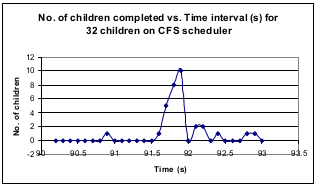
\includegraphics[width=0.45\textwidth]{pictures/fairness_32_cfs.png}
	\caption{Fairness-Messung für 32 Kinprozesse im CFS Scheduler.}
	\label{fig:fair_meas_cfs}
\end{figure}
\begin{figure}[h]
 	\centering
 	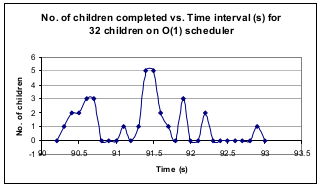
\includegraphics[width=0.45\textwidth]{pictures/fairness_32_O1.png}
 	\caption{Fairness-Messung für 32 Kinprozesse im O(1) Scheduler.}
 	\label{fig:fair_meas_o1}
\end{figure}
 
\begin{figure}[h]
 	\centering
 	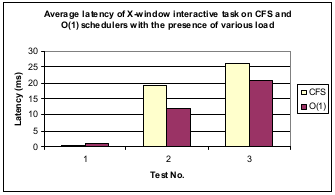
\includegraphics[width=0.45\textwidth]{pictures/avg_latency.png}
 	\caption{Durchschnittslatenz in CFS und O(1) Scheduler.}
 	\label{fig:avg_latency}
\end{figure}

\begin{figure}[h]
 	\centering
 	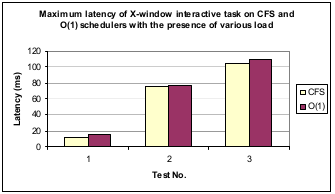
\includegraphics[width=0.45\textwidth]{pictures/max_latency.png}
 	\caption{Durchschnittslatenz in CFS und O(1) Scheduler.}
 	\label{fig:max_latency}
\end{figure}

\section{Zusammenfassung}

% Eine neue Spalte anfangen mit
\pagebreak

% Bibliographie entweder direkt hier eingeben (nur im Notfall)...
%\begin{thebibliography}{9}
%\bibitem{acmcategories}
%How to classify works using ACM's computing classification system.
%\newblock \url{http://www.acm.org/class/how_to_use.html}.
%
%\bibitem{Ivory2001}
%M.~Y. Ivory and M.~A. Hearst.
%\newblock The state of the art in automating usability evaluation of user
%  interfaces.
%\newblock {\em ACM Comput. Surv.}, 33(4):470--516, 2001.
%
%\end{thebibliography}

% ... oder die Bibliographie mit Hilfe von BibTeX generieren,
% dies ist auf jeden Fall die bessere Lösung und sollte nach
% Möglichkeit immer verwendet werden:
\bibliographystyle{abbrv}
\bibliography{literatur} % Daten aus der Datei literatur.bib verwenden.

\end{document}
